% here the evidence that the claims are correct is presented
% the structure, about 3 paragraphs for each analysis
% 1 This is my analysis
% 2 This analysis shows/demonstrates x
% 3 x supports my claim in the following way
\section{The Details}
\label{the_details}
% begin by describing what our implementation is
% answer the question, "what did you do"
In order to answer the question of
whether or not touch screen interactions may be used
in order to distinguish between users
a system is implemented to gather and analyze data
from interactions with the touchscreen of an Android device.
This data consists of location, pressure, and time
values associated with user's interactions with a soft keyboard.
%
For gathering purposes,
a keyboard application was modified to record
the necessary data values.
%
Two users were enlisted to acquire a large 
amount of data on two different Nexus 7 tablets.
In effect this creates four user, device combinations.
%
In order to analyze the collected data,
the system described in \ref{the_solution}
has been constructed.

% describe how the results were analyzed
The data were analyzed by 
%TODO 

%TODO move these figures to where they need to go in the paper
% describes how the Markov model will look after it has been constructed
\begin{figure}
\centering
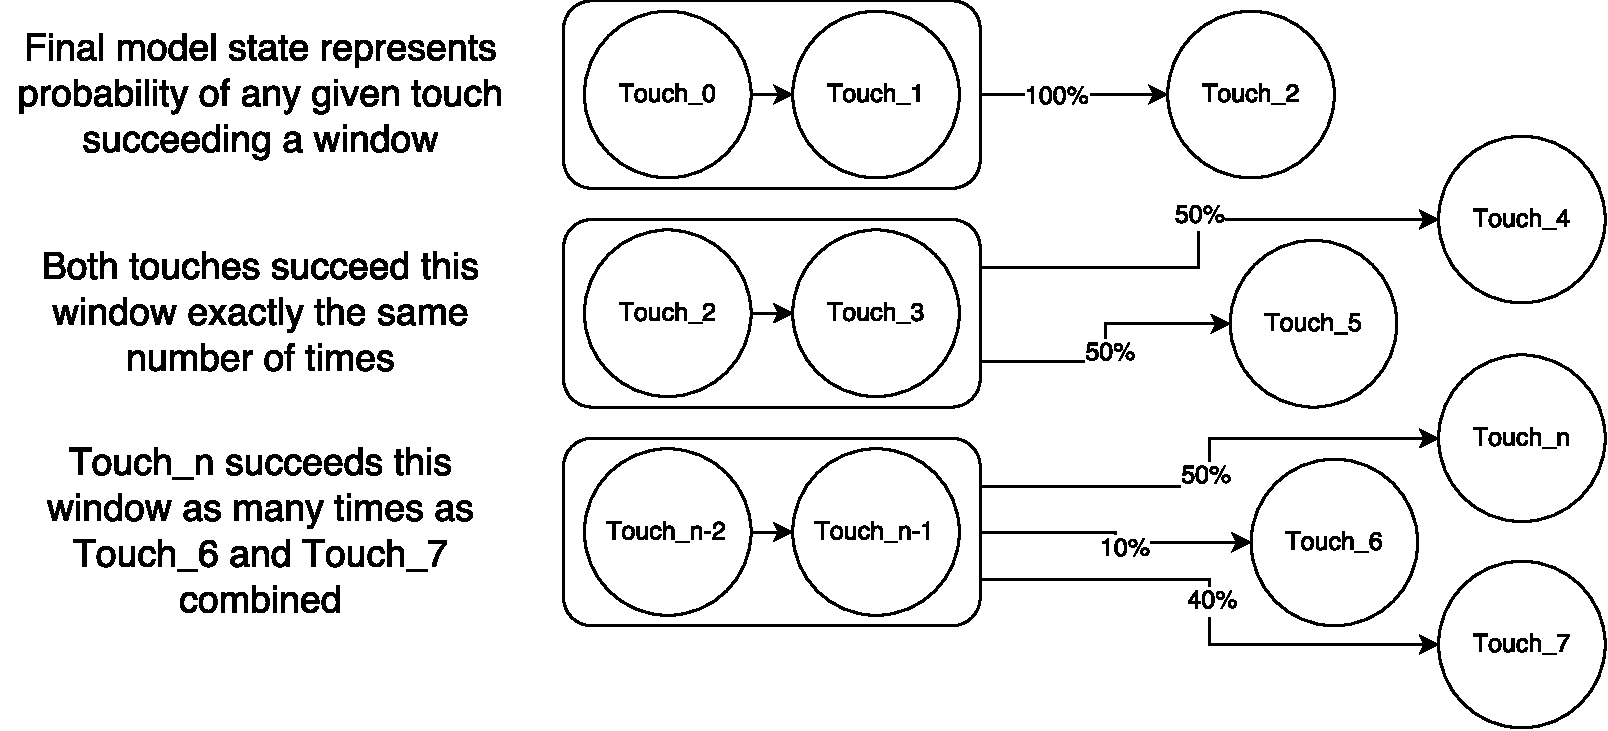
\includegraphics[width=.45\textwidth]{final_marcov_model_state.pdf}
\caption{
Example 2-Markov model after the probabilities have been calculated.
The rounded rectangles indicate 
a sequence of touch interactions 
which precede the following touch interaction with some probability $p$.
$p$ for token $T$ after sequence $W$ is computed 
as occurrences of $T$ after $W$
by occurrences of $W$.
% The top window states that 
% Touch\_2 succeeds the sequence Touch\_0, Touch\_1 with probability $100$\%.
}
\label{fig:final_markov_model_state}
\end{figure}

% show the range over which tokens are created
\begin{figure}
\centering
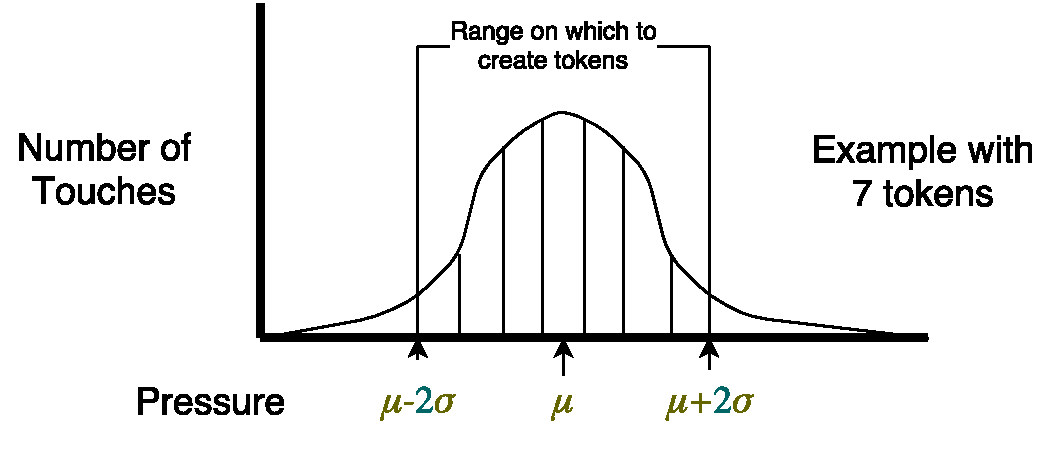
\includegraphics[width=.45\textwidth, keepaspectratio]{token_creation.pdf}
\caption{
Tokens are only created for 
pressure range $\mu \pm 2\sigma$ 
for each key.
Touches with pressure values
$p>\mu + 2\sigma$ and $p<\mu - 2\sigma$
are thrown out.
This eliminates outliers creating
increased reproducibility.
}
\label{fig:token_creation}
\end{figure}

% shows the pressure density for one of our users
\begin{figure}
\centering
%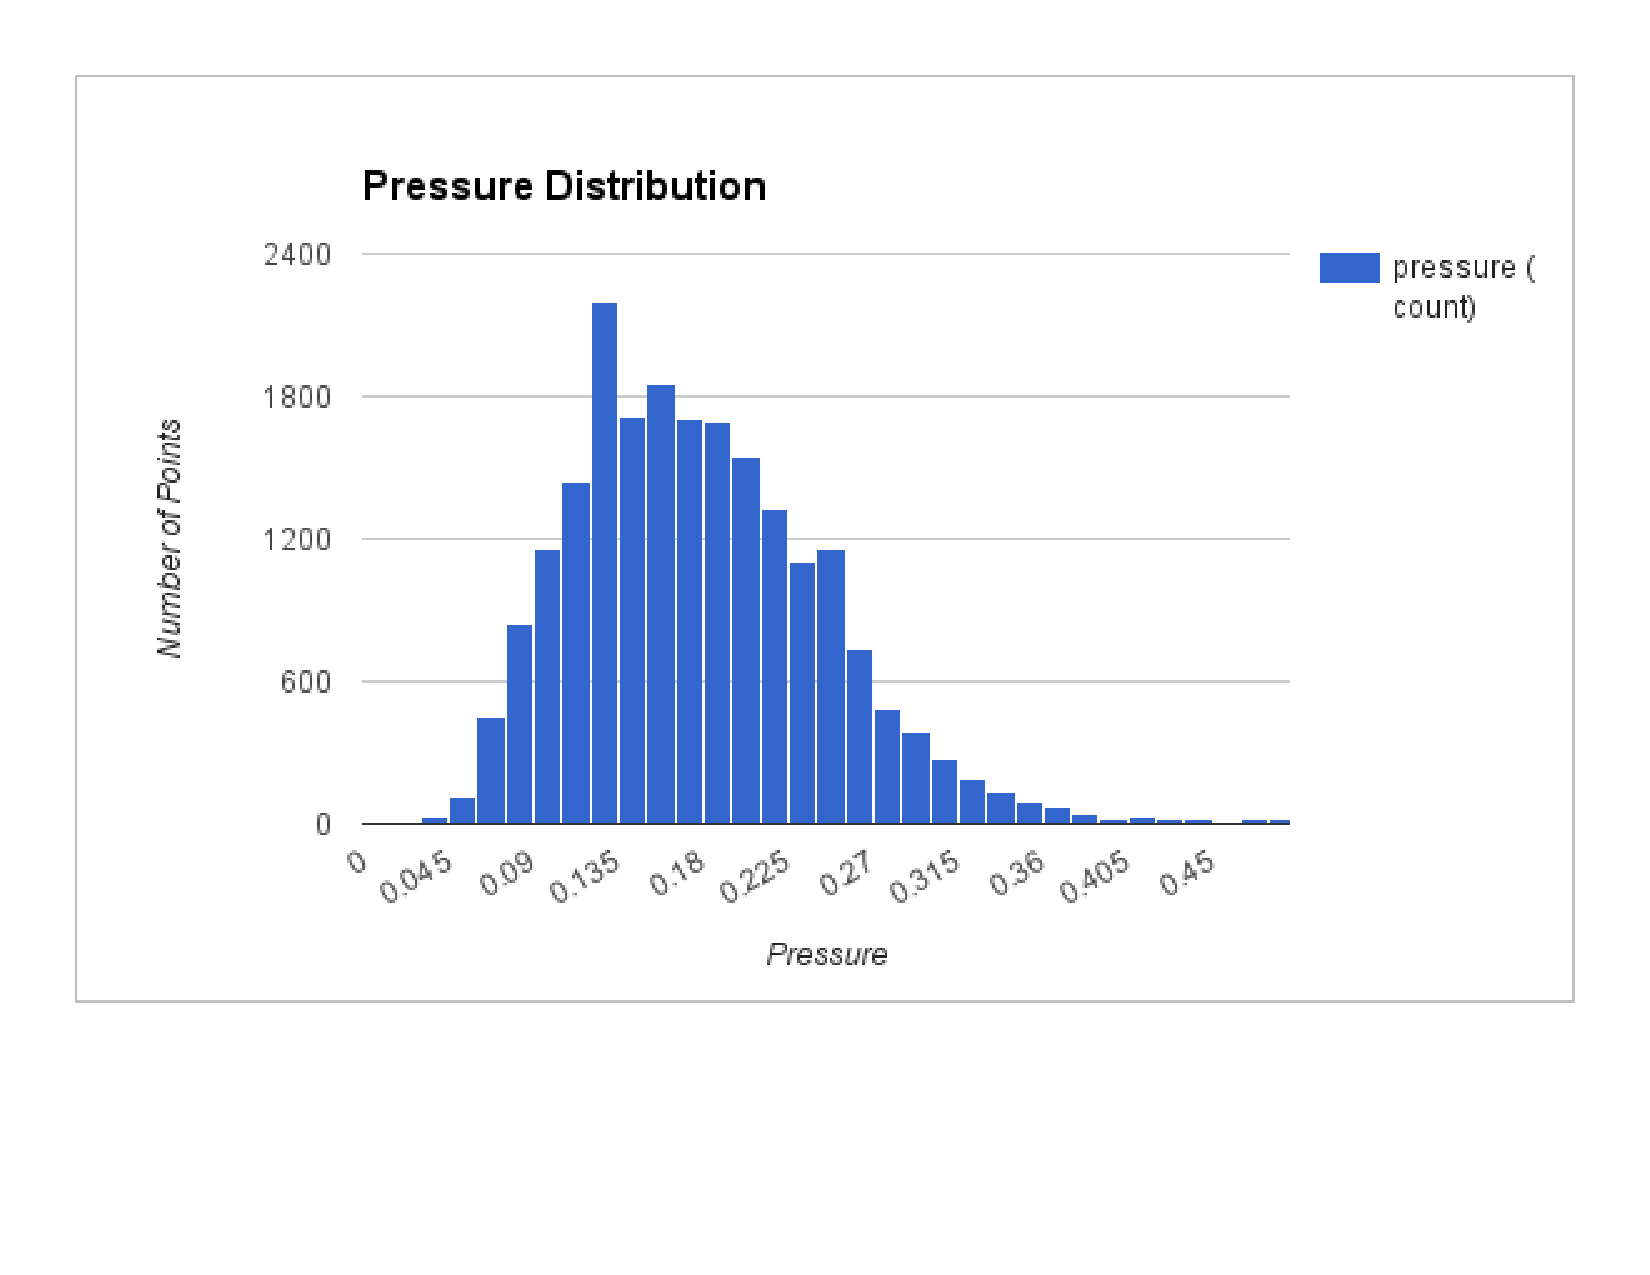
\includegraphics[width=.45\textwidth, keepaspectratio]{pressure_distribution.pdf}
\includegraphics[page=2, width=.45\textwidth, keepaspectratio]{Rplots.pdf}
\caption{
Density of touchscreen interactions' pressure values for one user.
%TODO say what is important about this observation
}
\label{fig:normal_distribution}
\end{figure}

% shows the qq-plot
\begin{figure}
\centering
%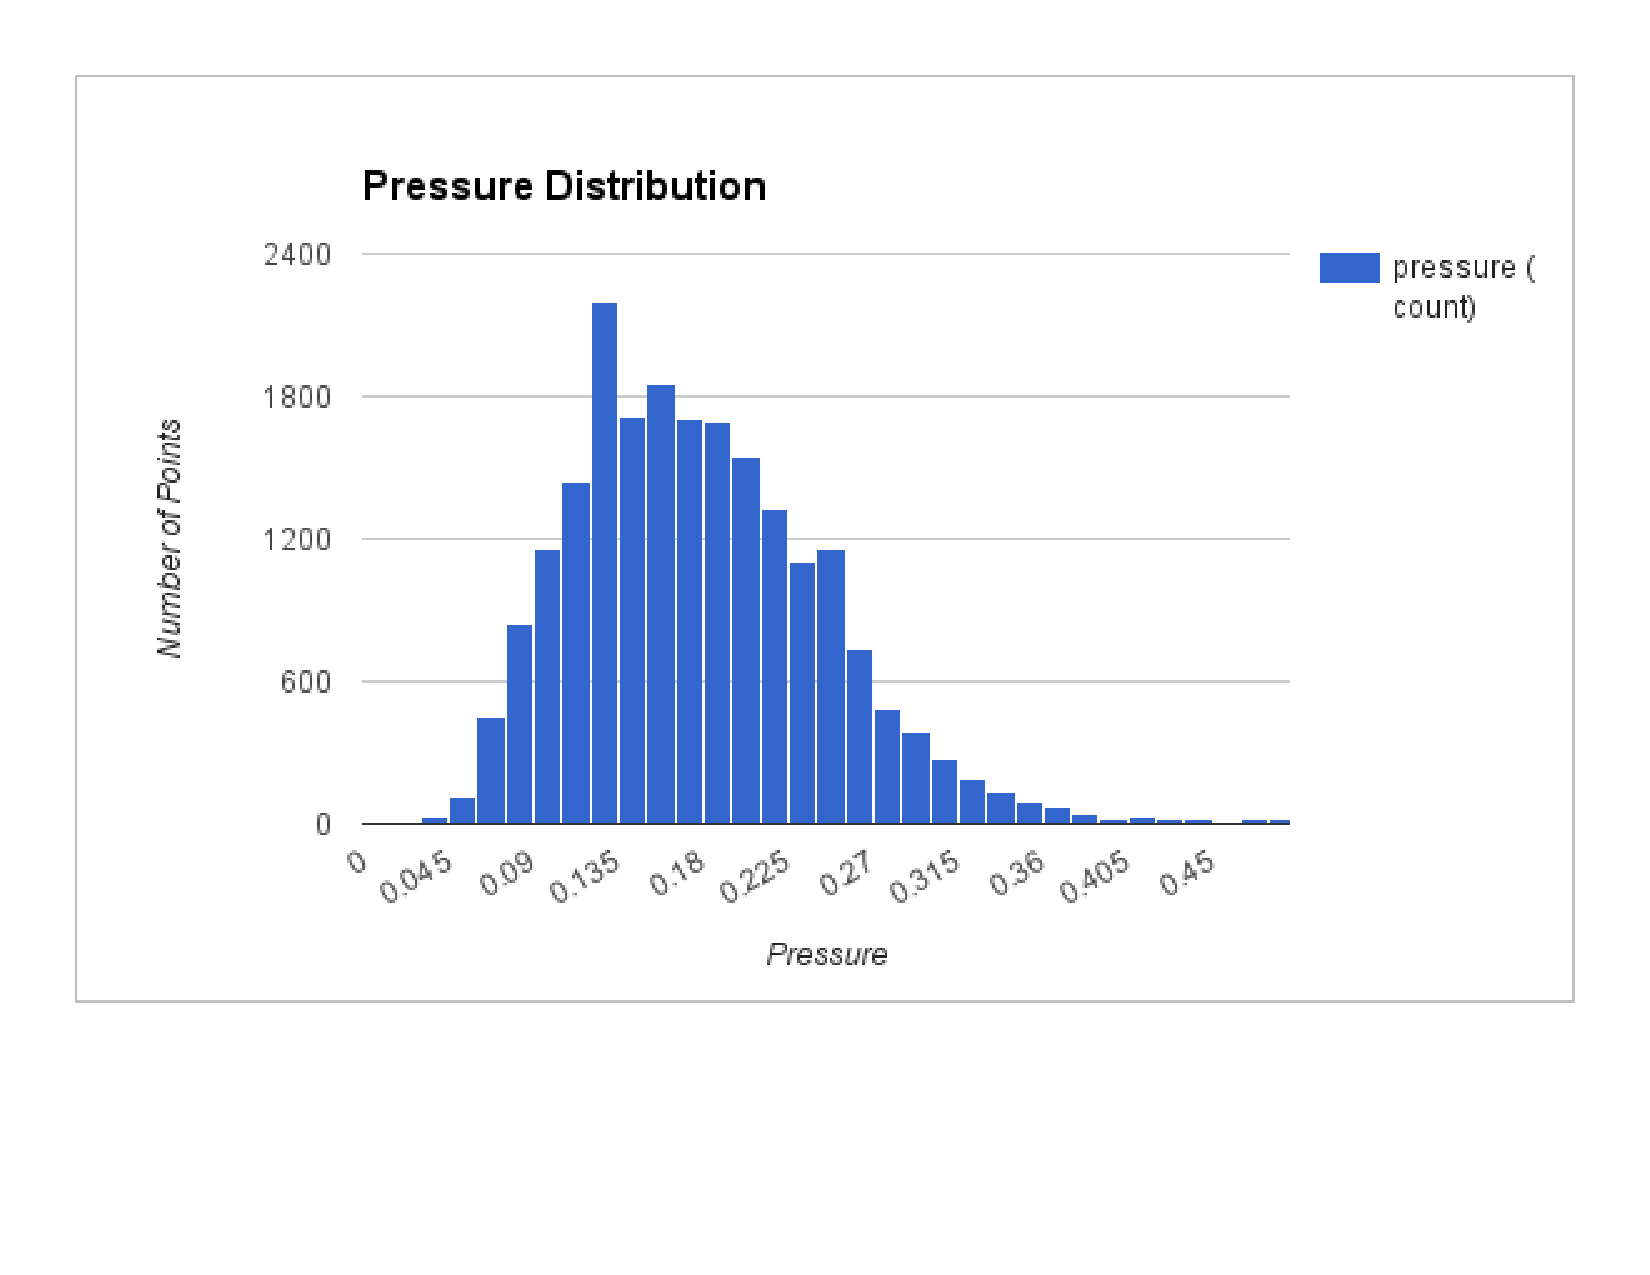
\includegraphics[width=.45\textwidth, keepaspectratio]{pressure_distribution.pdf}
\includegraphics[page=4, width=.45\textwidth, keepaspectratio]{Rplots.pdf}
\caption{
This Q-Q Plot describes data from
a data set having a right skew compared to normally distributed data.
}
\label{fig:qq_plot}
\end{figure}

% visually drive the process of token creation
% this shows a model with k=3
\begin{figure}
\centering
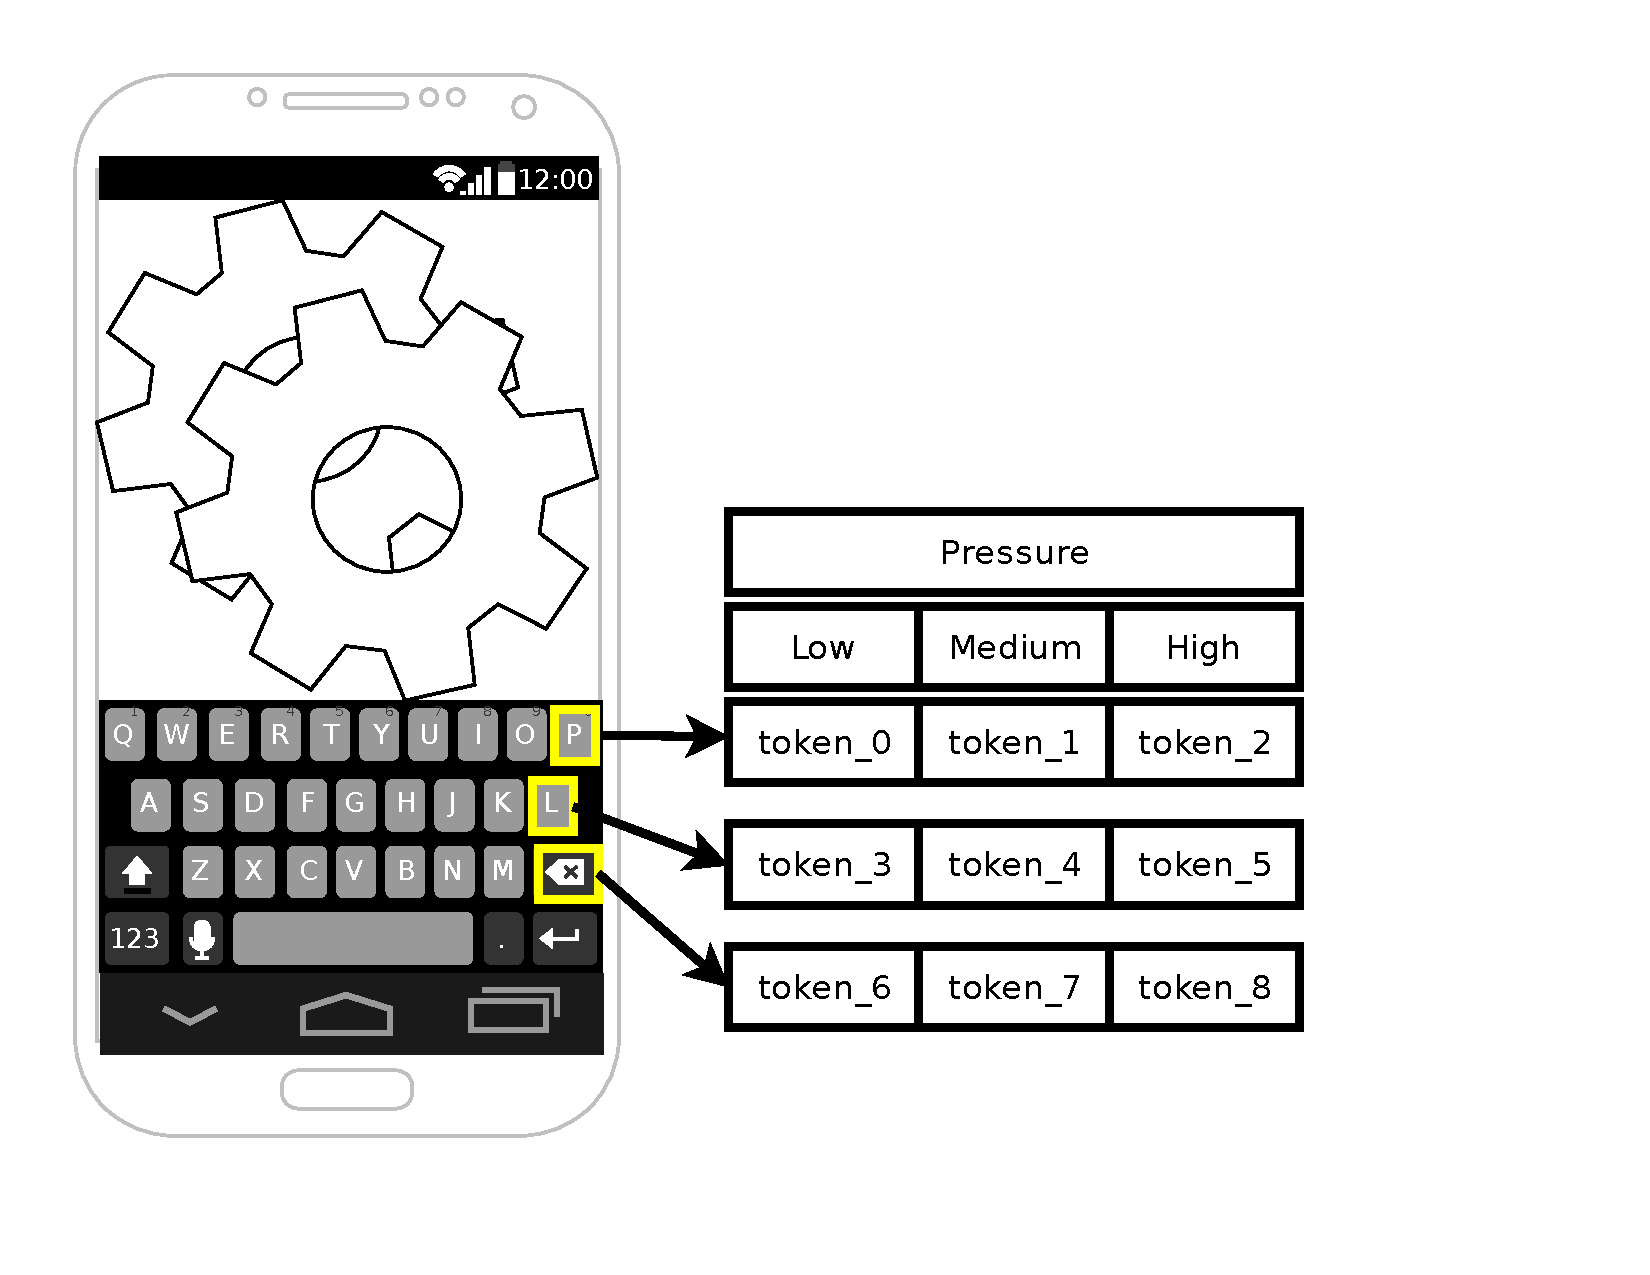
\includegraphics[width=.45\textwidth, keepaspectratio]{phone_tokens.pdf}
\caption{
Multiple tokens, $k=3$ above, correspond to each key location.
A touch screen interaction is assigned a token based on
key location and pressure.
}
\label{fig:phone_tokens}
\end{figure}

%TODO redo this figure's caption
\begin{figure}
\centering
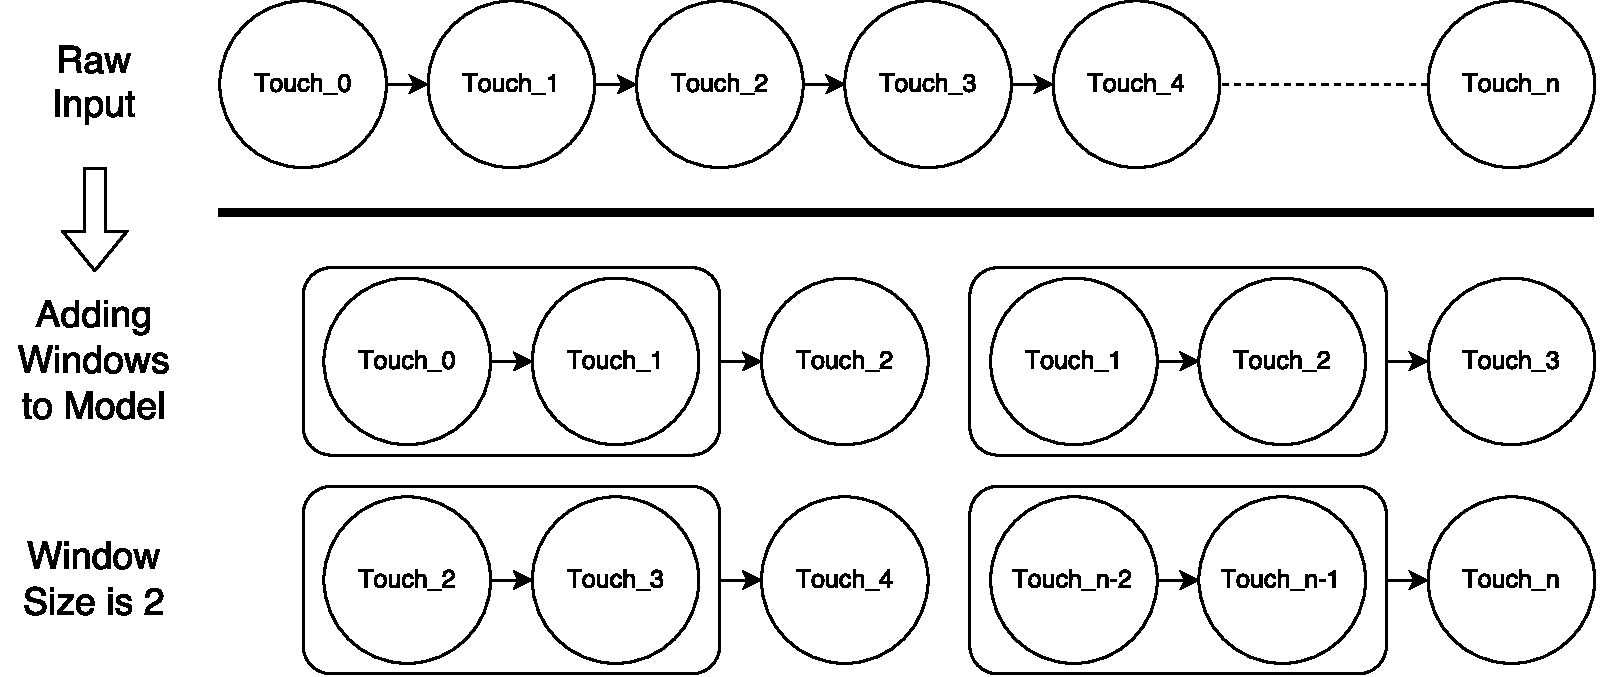
\includegraphics[width=.45\textwidth]{marcov_model_building.pdf}
\caption{
The top of this figure depicts the raw touchscreen interaction sequence.
Each touch represents a single interaction between the human user and the soft keyboard.
The diagram's lower portion demonstrates how the raw input is parsed into a 2-Markov model.
The bottom left image can be interpreted to say that Touch\_4 succeeds the sequence Touch\_2, Touch\_3 with some probability $p$.
}
\label{fig:markov_model_building}
\end{figure}

%basically the authentication scheme used
%frame it in more general terms, independent of our specific application
%\section{Differentiating \\A User-Device Pair}
\section{User-Device Pair Discrimination}
\label{sec:differentiation}
%TODO describe each of the model parameters in detail
%TODO state how each of the best model parameters were determined

%this figure describes how false positive and false negative percentages vary based on authentication threshold
\begin{figure}
\centering
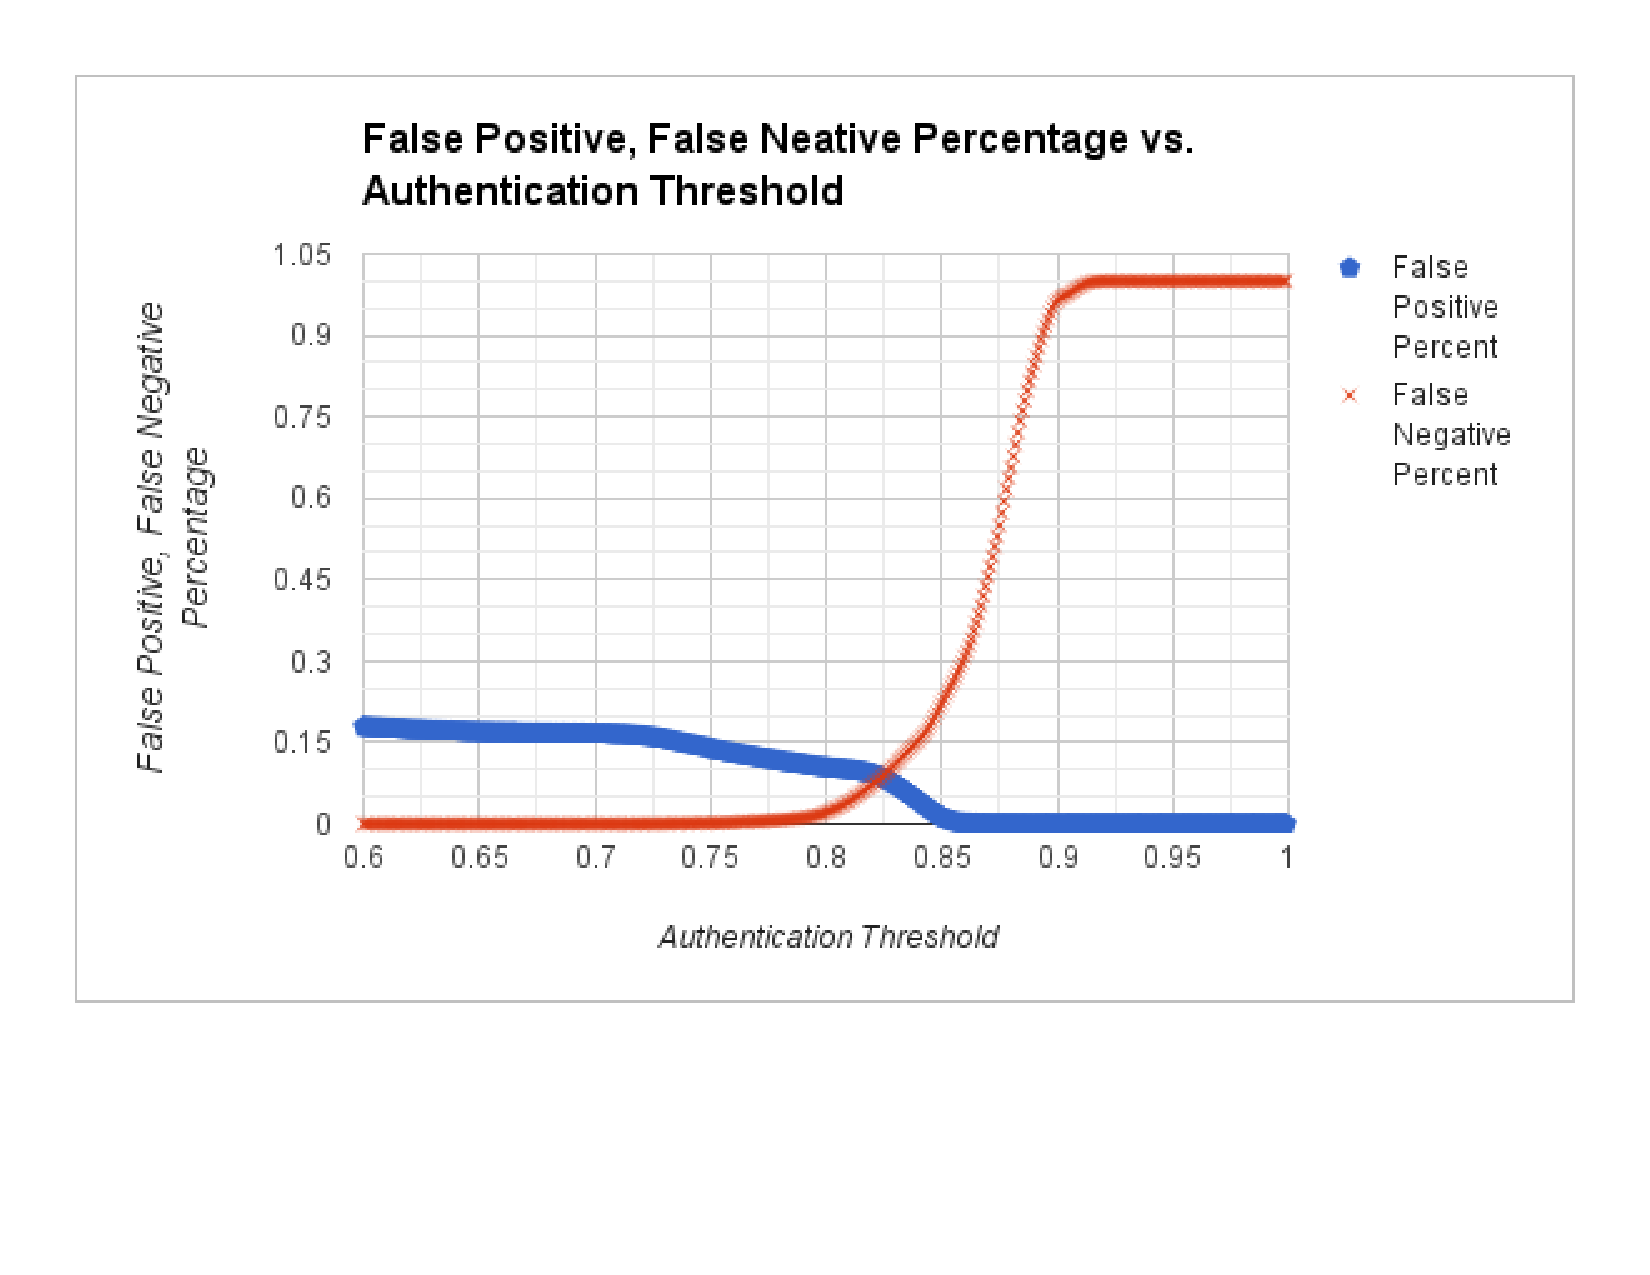
\includegraphics[width=.45\textwidth]{false_positive_vs_authentication_threshold.pdf}
\caption{False positive and false negative percentages vary as the authentication threshold is adjusted.}
\label{fig:threshold_vs_percentages}
\end{figure}

% this figure describes the effect of window size on authentication accuracy
\begin{figure}
\centering
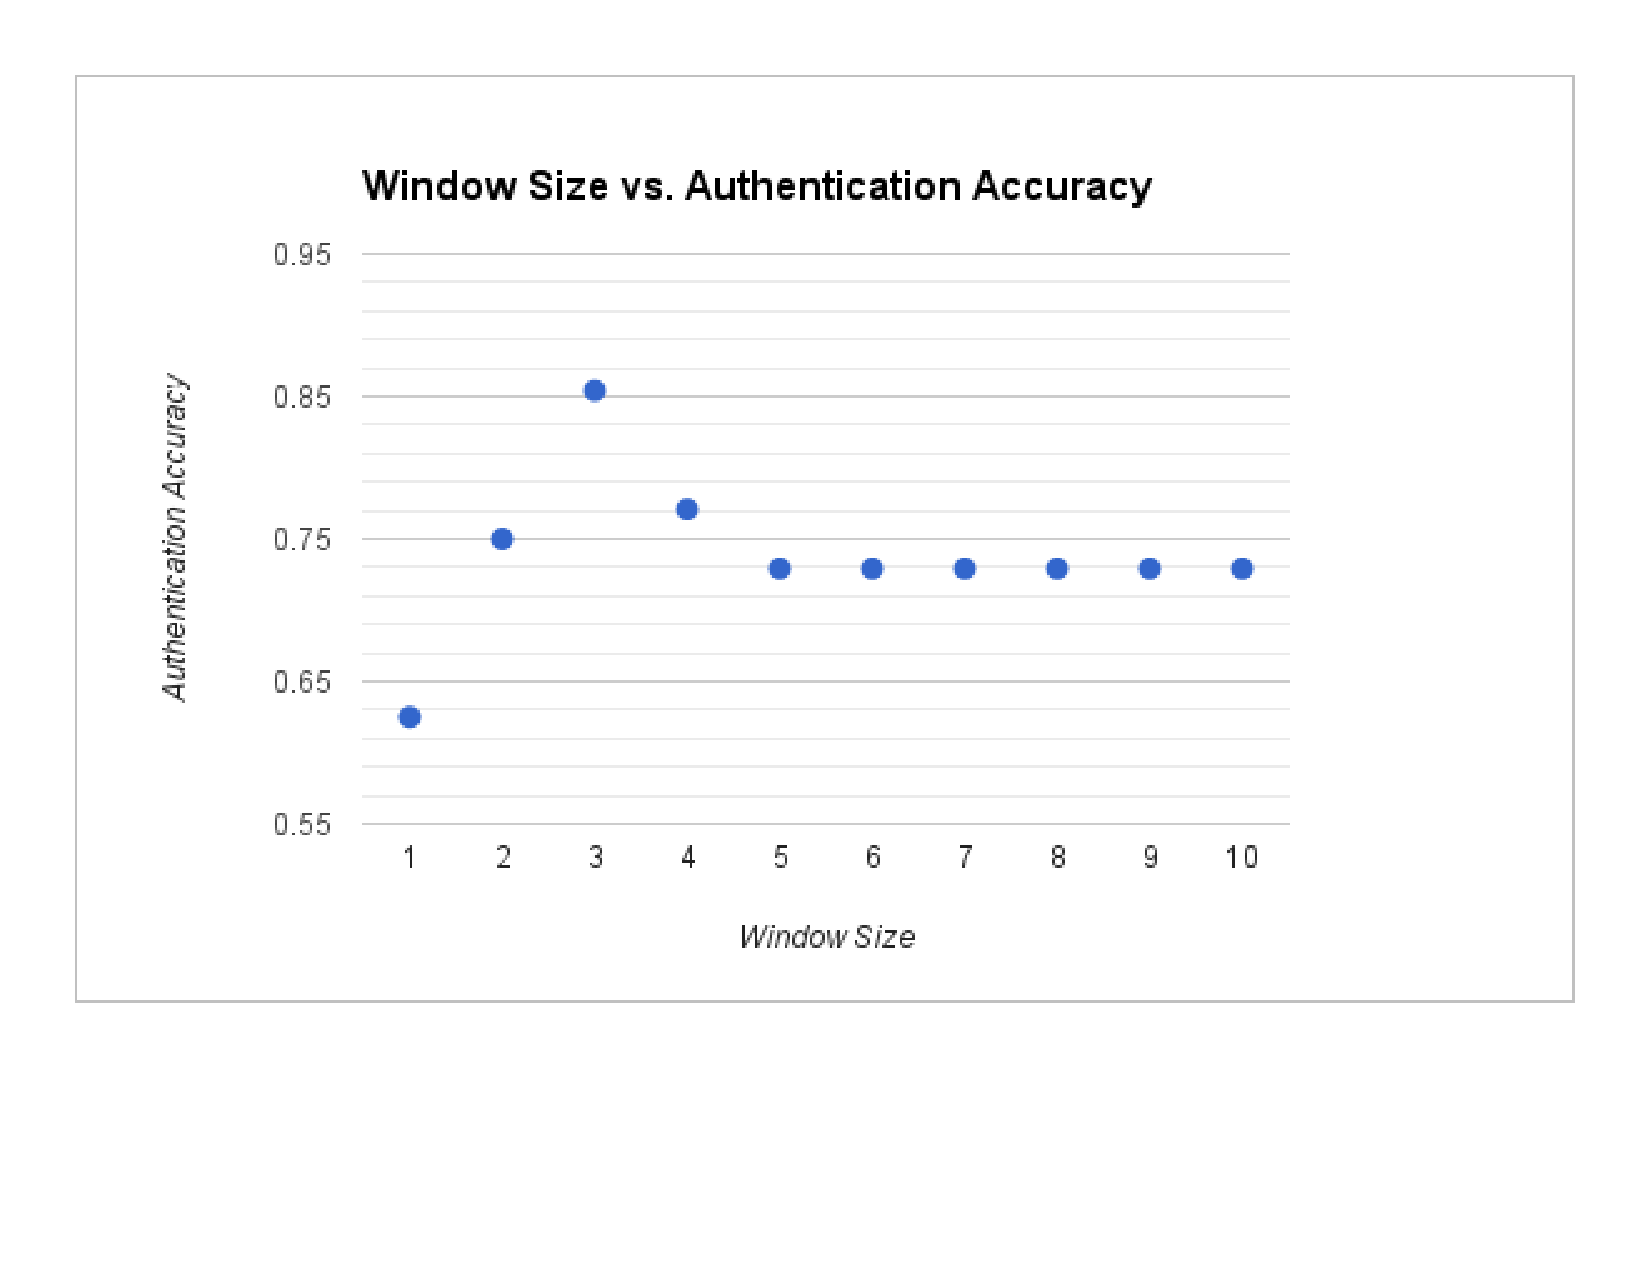
\includegraphics[width=.45\textwidth]{window_size_vs_authentication_accuracy.pdf}
\caption{The effect of $n$ in $n$-Markov Model window size on authentication accuracy.}
\label{fig:window_size_vs_authentication_accuracy}
\end{figure}

\begin{figure}
\centering
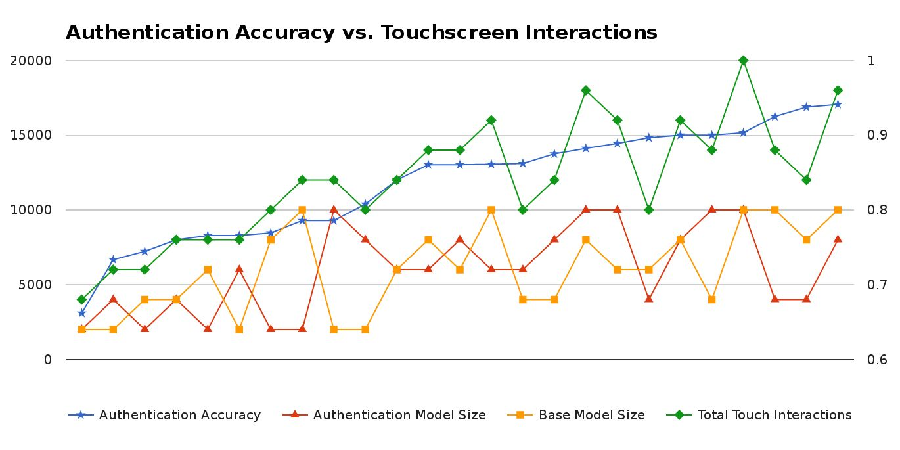
\includegraphics[width=.45\textwidth]{authentication_accuracy_vs_touchscreen_interactions.pdf}
\caption{
The left y axis describes the size of model
in number of touchscreen interactions.
We compare
authentication accuracy(blue star), measured on the right y axis, 
to authentication model size(red triangle),
base model size(yellow square),
and total touch interactions(green diamond)
measured on the left y axis.
Total touch interactions is the sum of
base model size and authentication model size.
}
\label{fig:authentication_accuracy}
\end{figure}

% describes authentication accuracy dependence on the amount of user data
\begin{figure}
\centering
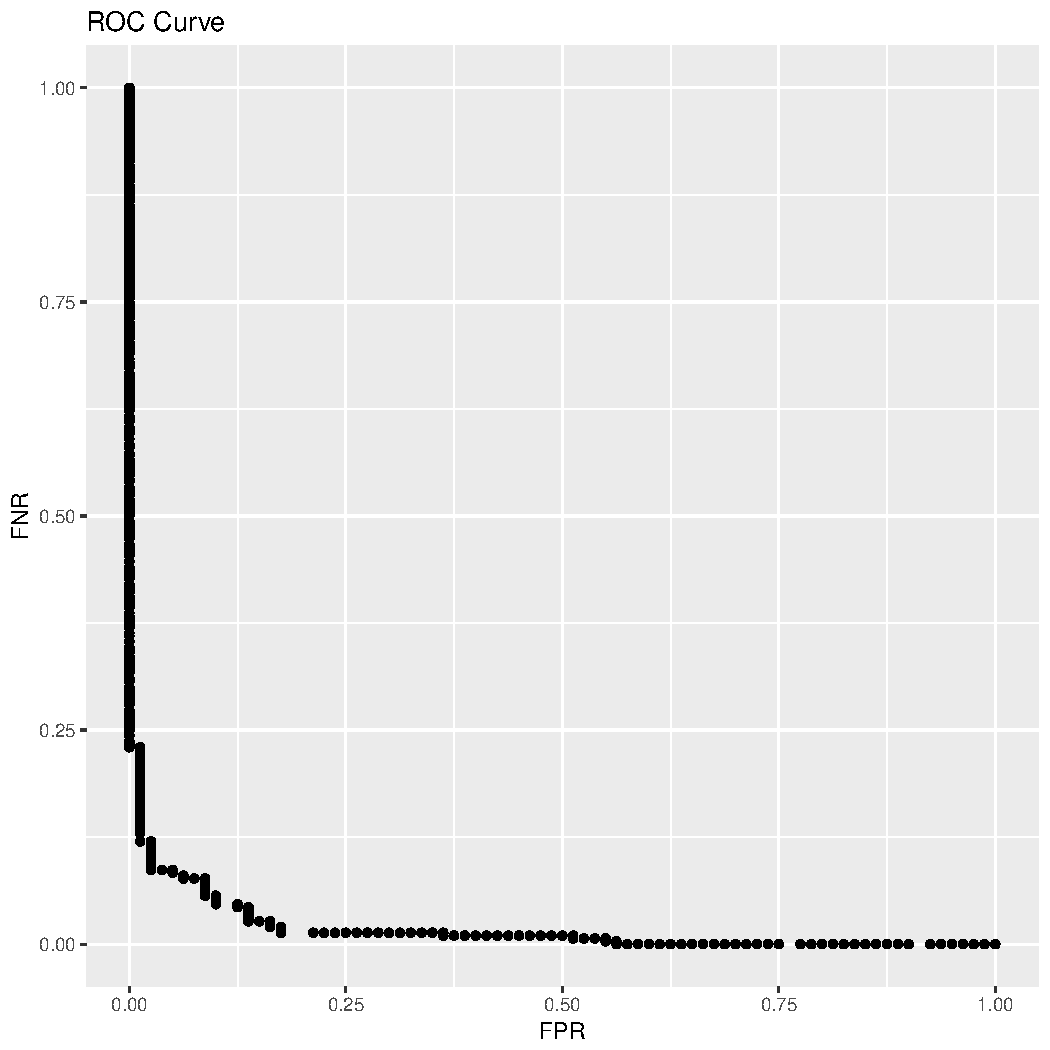
\includegraphics[width=.45\textwidth]{authentication_accuracy_vs_total_interactions.pdf}
\caption{
Authentication accuracy can be seen as
a function of
the total number of touch screen interactions
used in model construction.
Total touch interactions is the sum of
base model size and authentication model size.
}
\label{fig:total_touches_vs_authentication_accuracy}
\end{figure}

\begin{figure}
\centering
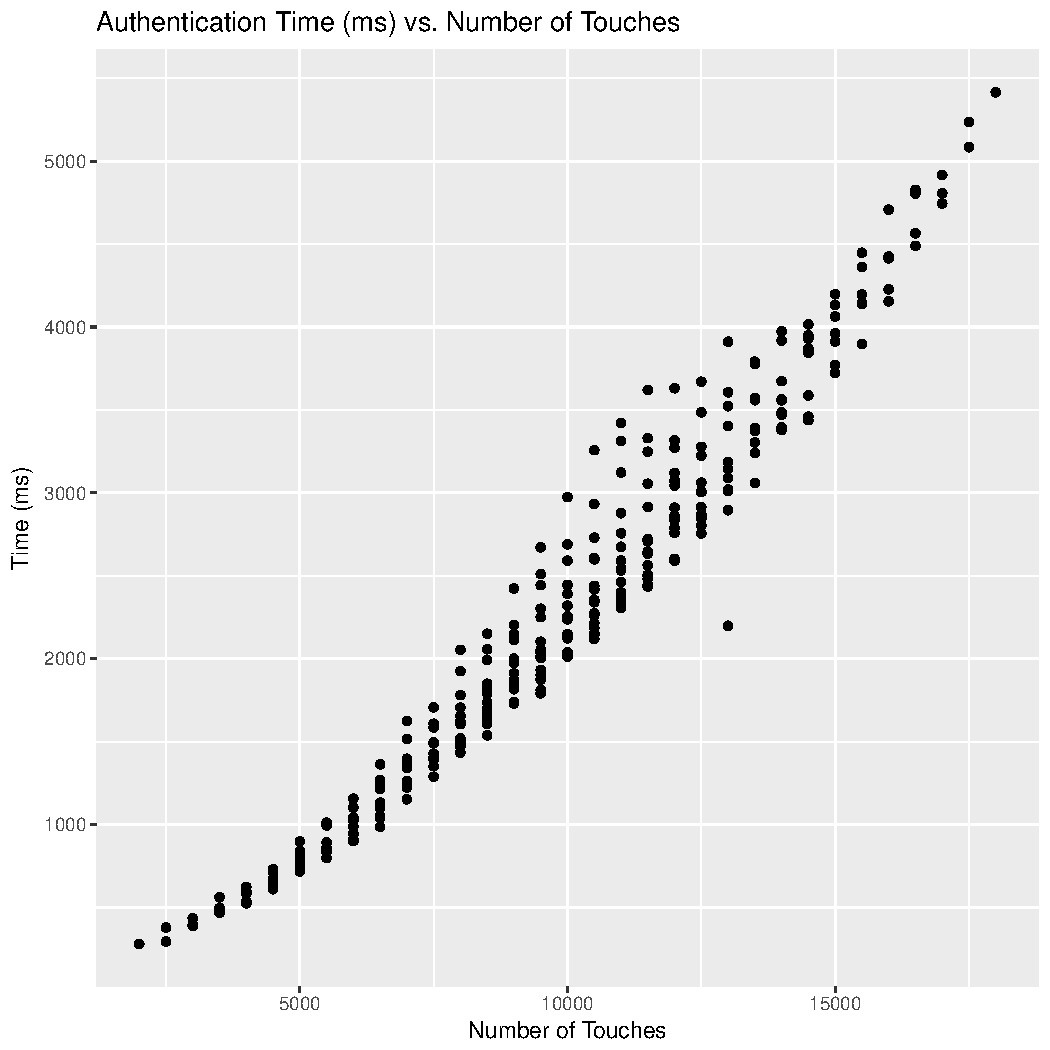
\includegraphics[width=.45\textwidth]{nexus_7_runtimes.pdf}
\caption{
The computation time, measured in seconds(sec), on a Nexus 7 tablet is
a function of
$Total Size =$ {\it base\_model\_size} $+$ {\it auth\_model\_size}.
Model sizes are measured by number of touch interactions used in their construction.
}
\label{fig:nexus_total_size_time}
\end{figure}



% %TODO move the following graphics to where they are useful,
% % use them to describe some aspect of the results
% \begin{figure}[htb]
% \caption{}
% \begin{center}
% 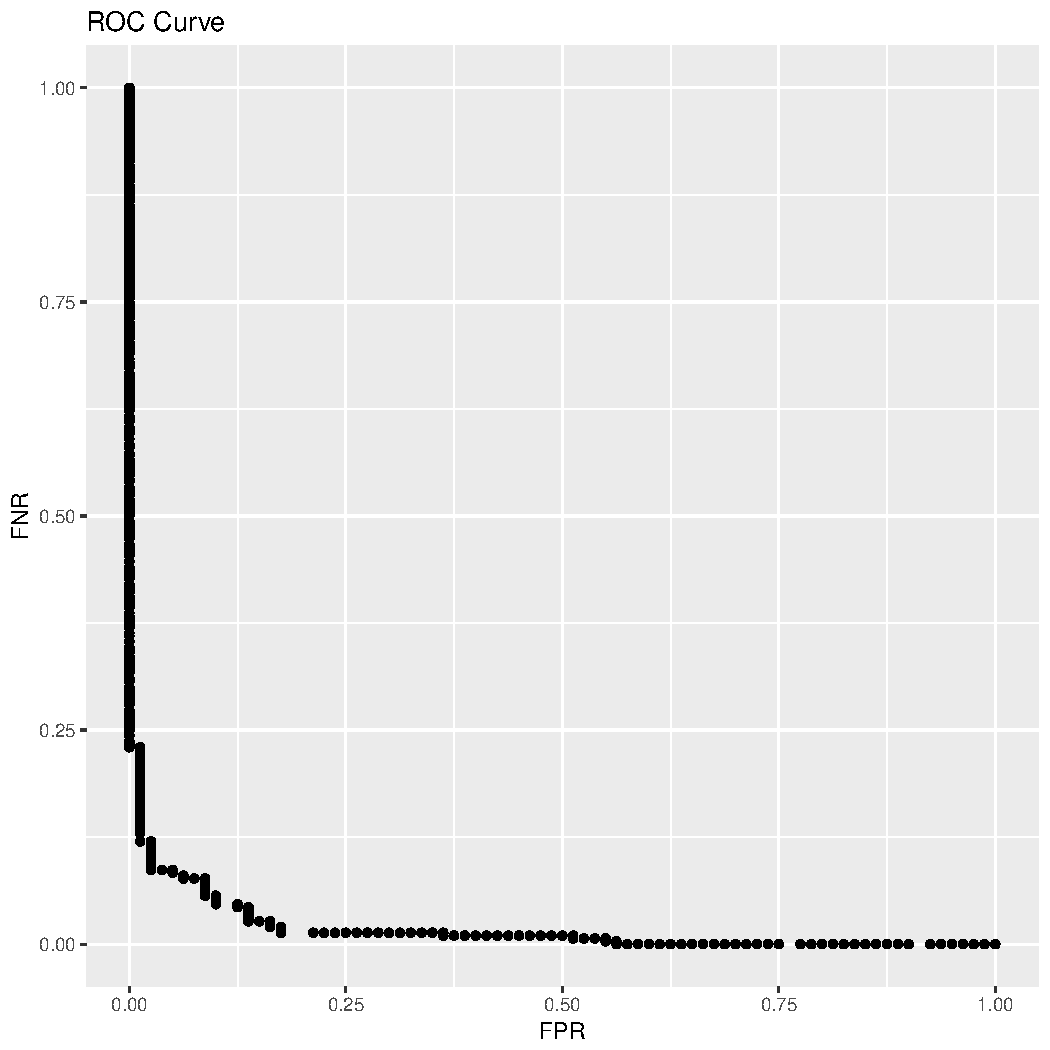
\includegraphics[keepaspectratio=true,width=0.45\textwidth]{authentication_accuracy_vs_total_interactions.pdf}
% \label{figure_authentication_accuracy}
% \end{center}
% \end{figure}

% \begin{figure}[hbt]
% \caption{}
% \begin{center}
% 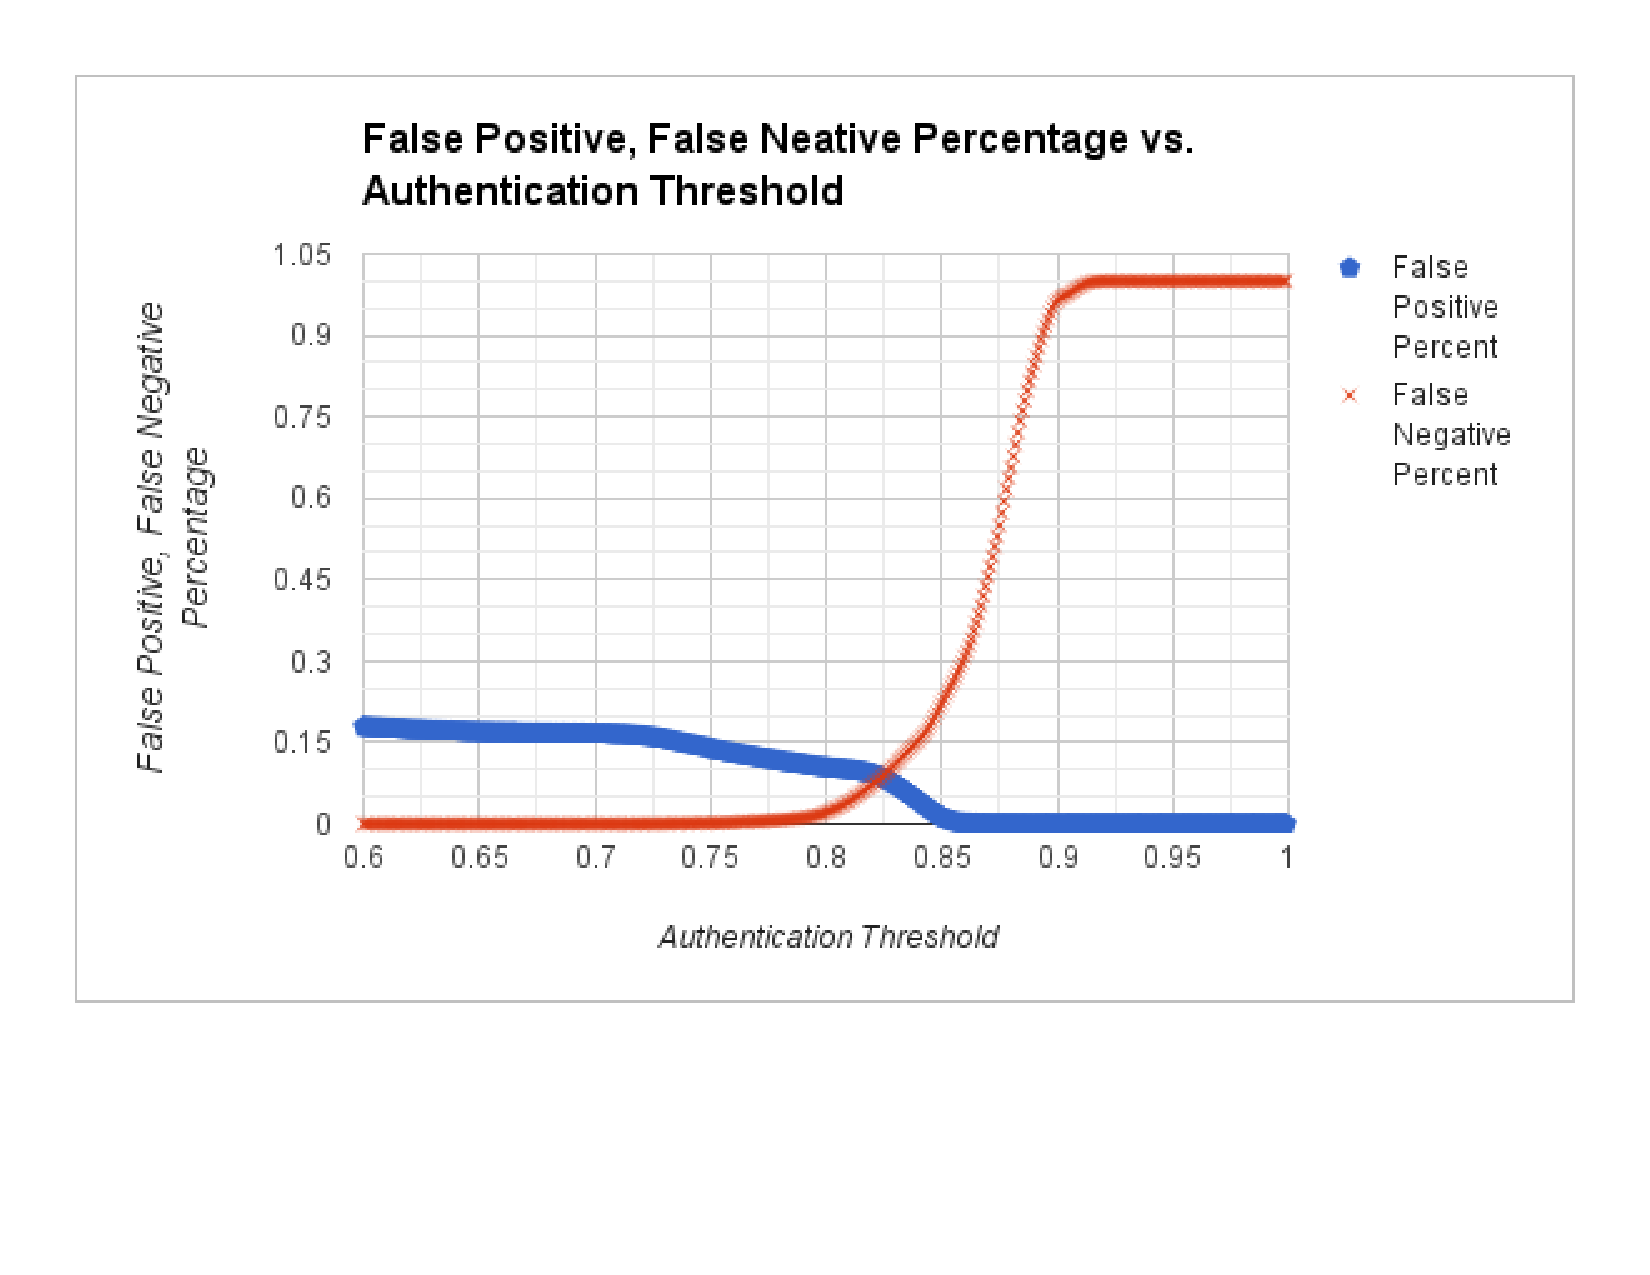
\includegraphics[keepaspectratio=true,width=0.45\textwidth]{false_positive_vs_authentication_threshold.pdf}
% \label{figure_false_positive}
% \end{center}
% \end{figure}

% \begin{figure}[hbt]
% \caption{}
% \begin{center}
% 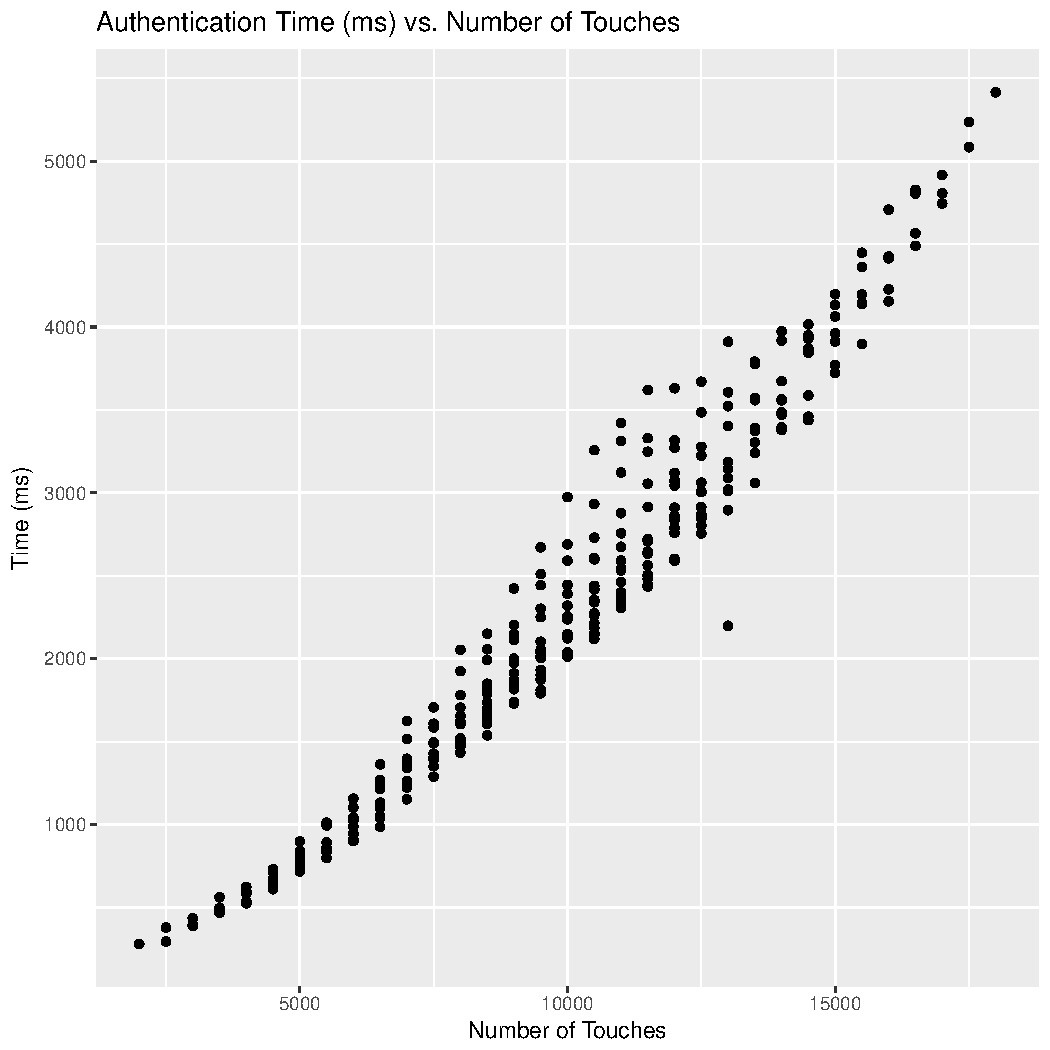
\includegraphics[keepaspectratio=true,width=0.45\textwidth]{nexus_7_runtimes.pdf}
% \label{figure_nexus_7_runtimes}
% \end{center}
% \end{figure}

\lipsum[0-8]

% include mention of some problems which presented themselves
Some notable problems presented themselves
throughout the course of this work
which could influence the usability of such a 
system in a practical sense.
%
The Android \textbf{MotionEvent} class \textbf{getPressure()} method
used to collect pressure data in our system
does not always return a high granularity of values.
The pressure values are sometimes grouped
into large steps.
There might, for example,
be $8$ steps between $0.0$ and $1.0$ on some devices.
This is a problem for our system which uses
these pressure values to understand user variability.
%
The problem seems to be device dependent
suggesting that the device drivers may have a role to play
in decreasing the reported graininess of pressure.
Another possibility might be the values
reported by the sensors,
Perhaps these sensors only report a small number of steps.
%TODO state the performance impact on our system

% tie all analysis's back to the claims
%TODO